\documentclass[12pt, oneside]{report}

%Debugging packages and commands:
%\usepackage{showframe}
\overfullrule=10pt

% Modular Compilation
\usepackage{subfiles}
\providecommand{\main}{.}

% LETU Thesis Formatting
\usepackage{\main/letuThesis}
\usepackage[crop=pdfcrop]{pstool}
\usepackage{standalone} % for inputting tikz pictures

% External Packages
\usepackage{lipsum}

% Preamble Information
\title{Real-Time \\ Model Predictive Control}
\author{Jeremy Goossen}
\committee{
	Dr. G. Nathan Green, PhD \\
	Dr. Joonwan Kim, PhD \\
	Dr. Marian Iordache, PhD \\
	Dr. Andrew Davis}
\university{LeTourneau University}
\school{School of Engineering and Engineering Technology}
\discipline{Electrical Engineering}
\titlepageauthor{J. Goossen}
%\lastChapter{}

\usepackage[hidelinks]{hyperref}
\begin{document}

\frontmatter

\maketitle
\makesignatures
\makecopyright

\unpacklipsum[1-3]
\makeabstract{\lipsumexp}

\makeacknowledgments{\lipsum[4-5]\par
I'd like to acknowledge everyone who made this possible. Thanks!\par}

\tableofcontents

%\clearpage
%\addcontentsline{toc}{chapter}{List of Tables}
%\chapter*{List of Tables}
\listoftables

%\clearpage
%\addcontentsline{toc}{chapter}{List of Figures}
%%\addtocontents{lof}{~\hfill Page\par}
\listoffigures





\mainmatter % Switch to Arabic numbering

\chapter{Introduction}
\lipsum[1]
%\section{Suspendisse vitae elit. Aliquam arcu neque, ornare in, ullamcorper quis, commodo eu, libero.} % \lipsum[10][1-2]
\section{\lipsum[150][1-3]}
\lipsum[3]%
\footnote{This is simply the ubiquitous ``Lorem Ipsum'' placeholder text for typesetting. This is a long footnote, and extends to more than just a single line.}

\begin{figure}[h]
  \centering
  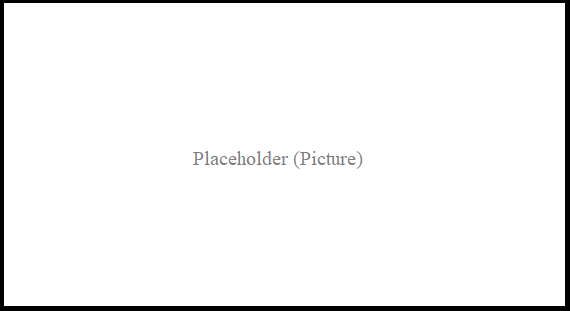
\includegraphics[width=.7\textwidth]{figures/pictures/placeholder}
  \caption{The caption of the figure}
  \label{fig:BlockDiagram1}
\end{figure}
  
\begin{figure}[h]
  \centering
  \includeplot[width=.8\textwidth]{figures/plots/placeholder}
  \caption{The caption of the figure which is much longer than the other captions, since it should flow to the next line every time}
  \label{fig:BlockDiagram2}
\end{figure}

\begin{figure}[h]
  \centering
  \includediagram{figures/diagrams/placeholder}
  \caption{The caption of the figure}
  \label{fig:BlockDiagram3}
\end{figure}

\begin{figure}[h]
  \centering
  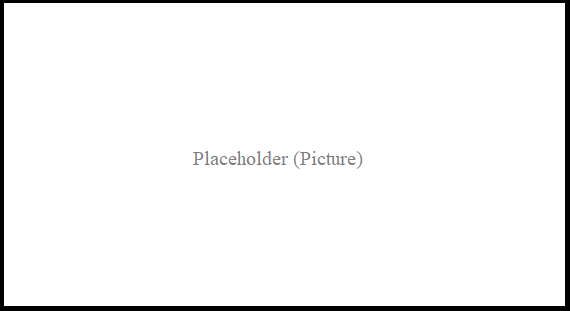
\includegraphics[width=0.5\textwidth]{figures/pictures/placeholder}
  \caption{The caption of the figure}
  \label{fig:BlockDiagram4}
\end{figure}

\begin{figure}[h]
  \centering
  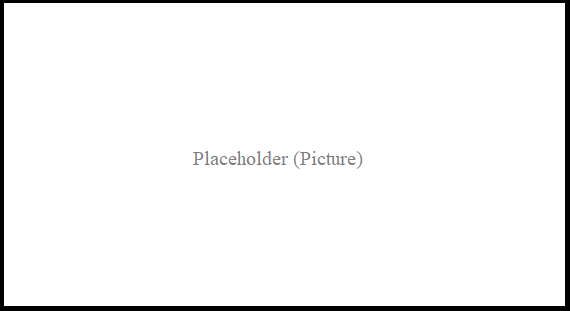
\includegraphics[width=0.5\textwidth]{figures/pictures/placeholder}
  \caption{The caption of the figure}
  \label{fig:BlockDiagram4}
\end{figure}

\begin{figure}[h]
  \centering
  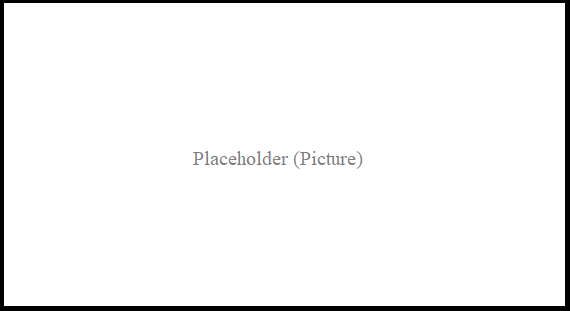
\includegraphics[width=0.5\textwidth]{figures/pictures/placeholder}
  \caption{The caption of the figure}
  \label{fig:BlockDiagram4}
\end{figure}

\begin{figure}[h]
  \centering
  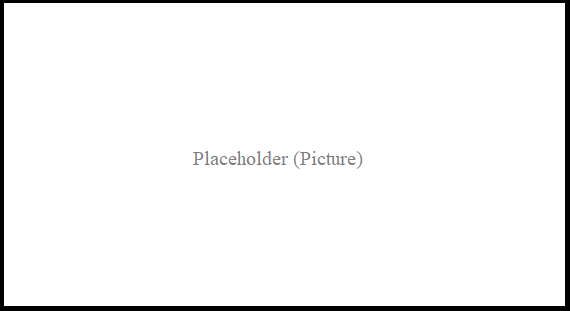
\includegraphics[width=0.5\textwidth]{figures/pictures/placeholder}
  \caption{The caption of the figure}
  \label{fig:BlockDiagram4}
\end{figure}

\begin{figure}[h]
  \centering
  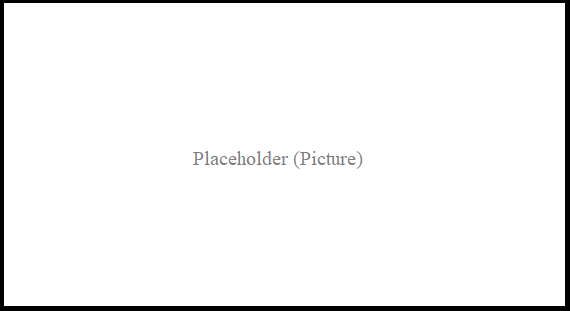
\includegraphics[width=0.5\textwidth]{figures/pictures/placeholder}
  \caption{The caption of the figure}
  \label{fig:BlockDiagram4}
\end{figure}

\begin{figure}[h]
  \centering
  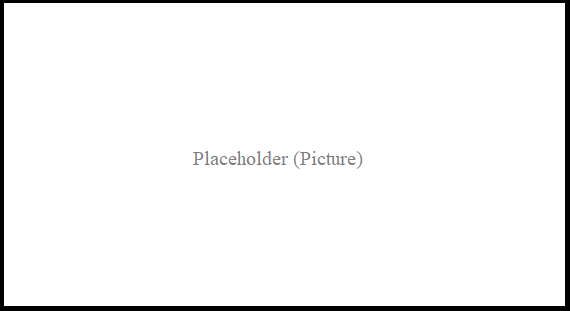
\includegraphics[width=0.5\textwidth]{figures/pictures/placeholder}
  \caption{The caption of the figure}
  \label{fig:BlockDiagram4}
\end{figure}

\begin{figure}[h]
  \centering
  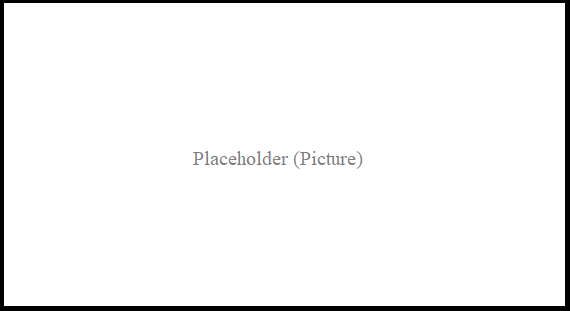
\includegraphics[width=0.5\textwidth]{figures/pictures/placeholder}
  \caption{The caption of the figure}
  \label{fig:BlockDiagram4}
\end{figure}

\begin{figure}[h]
  \centering
  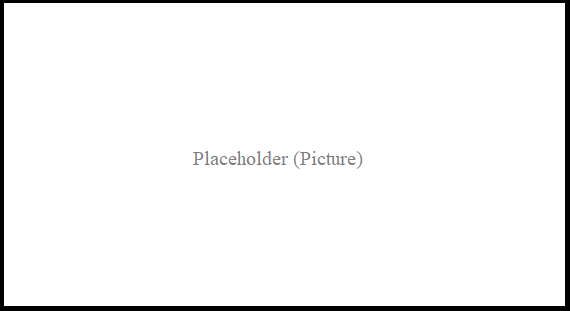
\includegraphics[width=0.5\textwidth]{figures/pictures/placeholder}
  \caption{The caption of the figure}
  \label{fig:BlockDiagram4}
\end{figure}


%This paragraph references Figure \ref{fig:BlockDiagram1}, and should be clickable.

\lipsum[4]%
\footnote{Another paragraph from the same source.}\footnote{And something else I remembered that merits its own footnote.}

\subsection{Subsection Title}
\lipsum[5]

\subsubsection{Sub-subsection}
\lipsum[6-7]
\subsubsection{Another Sub-subsection}
\lipsum[8-9]\footnote{This footnote is on a new page and is numbered starting from the beginning}

\section{\lipsum[150][4]}

\subsection{\lipsum[150][8]}
\lipsum[10]

\unpacklipsum[150][5]
\chapter{\lipsumexp}

\section{\lipsum[150][6]}
\lipsum[5-6]

\section{\lipsum[150][7]}
\lipsum[7]

\chapter{One}

This page contains a sample table.

\begin{thesistable}[htbp]
{c c c}
[A Simple Table]
{A Simple Table. Note that this table has some extra information added to the caption at this point in the text, but this extra text will not appear in the List of Tables.}
{tab:sampletable}
{First & Second & Third}
Data 1 & Data 2 & Data 3 \\
Data 4 & Data 5 & Data 6 \\
\end{thesistable}

\chapter{Another}
\chapter{Another}
\chapter{Another}
\chapter{Another}
\begin{figure}[h]
  \centering
  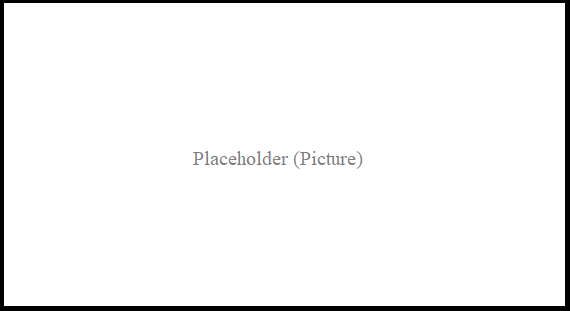
\includegraphics[width=0.5\textwidth]{figures/pictures/placeholder}
  \caption{The caption of the figure}
  \label{fig:BlockDiagram4}
\end{figure}
\chapter{Another}
\chapter{Another}
\chapter{Another}
\chapter{Another}
\chapter{Another}
\chapter{Another}
\chapter{Another}
\chapter{Another}



\backmatter

\bibliographystyle{ieeetr}
\bibliography{\main/references/references}


\begin{appendices}

\unpacklipsum[141][1-3]
\chapter{\lipsumexp}
\lipsum[140][4]

\begin{figure}[h]
  \centering
  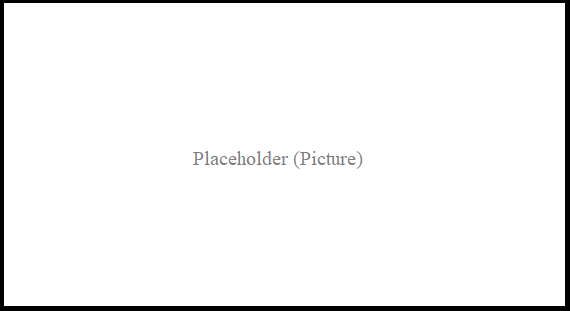
\includegraphics[width=0.5\textwidth]{figures/pictures/placeholder}
  \caption{The caption of the figure}
  \label{fig:BlockDiagram4}
\end{figure}

\section{\lipsum[140][3]}
\lipsum[8-9]

\section{\lipsum[140][5]}
\lipsum[10]

\unpacklipsum[140][6]
\chapter{\lipsumexp}
\lipsum[11] \cite{einstein, latexcompanion, knuthwebsite}


\end{appendices}






\end{document}